
\section{Felhaszn\'al\'oi dokument\'aci\'o}
\subsection{Feladat}
A program azt feladatot hivatott ell\'atni, hogy mikrofonbemenetr\"ol \'erkez\H o hangjelet feldolgozzon, majd ezt az eredm\'enyt vizu\'alisan megjelen\'itse. Mindezt \'ugy, hogy az id\H o ami eltelik a jel \'eszlel\'ese \'es az eredm\'eny megjelen\'ese k\"oz\"ott minim\'alis legyen.

A megjelen\'it\'es egy h\'aromdimenzi\'os spektogramon t\"ort\'enik. Ezen az $x$-tengelyen az id\H o, az $y$-tengelyen a frekvencia, a $z$-tengelyen pedig a hangban tal\'alt adott frekvenci\'aj\'u hull\'am amplit\'ud\'oja jelenik meg.

\subsection{Hangfeldolgoz\'as}
A jel feldolgoz\'asa vide\'ok\'arty\'an v\'egzett diszkr\'et Fourier-transzform\'aci\'oval t\"ort\'enik. A transzform\'aci\'o a hangjelet az id\H o f\"uggv\'eny\'er\H ol a frekvencia f\"uggv\'eny\'eve alak\'itja. 

Tekintettel arra, hogy a diszkr\'et Fourier-transzform\'aci\'o kifejezetten m\H uveletig\'enyes algoritmus ($\ordo{n^2}$) a gyakorlatban \'altal\'aban gyors Fourier-transzform\'ac\'iot haszn\'alnak az ilyen feladatok megold\'as\'ara, amellyel $\ordo{n\cdot\log n}$-re lehet ezt jav\'itani.

Azonban a processzorral ellent\'etben, ahol kevesebb mag van, de azok magasabb \'orajelen, a GPU-ban rengeteg sz\'am\'it\'asi egys\'eg van, amelyek egym\'ast\'ol f\"uggetlen\"ul p\'arhuzamosan tudnak m\H uk\"odni, viszont alacsonyabb \'orajelen. \'Igy ha a kimenet egyes  komponenseit k\"ul\"on sz\'am\'it\'asi egys\'eg sz\'amolja p\'arhuzamosan, akkor elm\'eletileg $\ordo{n}$-es m\H uveletig\'enyr\H ol besz\'elhet\"unk, ami m\'egink\'abb hozz\'aj\'arul a kis k\'es\'es\H u megjelen\'it\'eshez. 


\subsection{Technol\'ogi\'ak}
\subsubsection{Megjelen\'it\'es}
Az alkalmaz\'as egy darab megjelen\'it\H o ablakb\'ol \'all. Az ablakkezel\'es\'ert a ny\'ilt forr\'ask\'od\'u \href{http://www.glfw.org/}{GLFW} multi-platform k\"onyvt\'ar felel\H os.

TODO: k\'ep a fut\'asr\'ol

\subsubsection{Hangkezel\'es}
A mikrofon bemenet kezel\'es\'et a PortAudio cross-platform k\"onyvt\'ar v\'egzi. Ezt haszn\'alja t\"obbek k\"oz\"ott az \href{http://audacity.sourceforge.net}{Audacity} hangfelvev\H o \'es -v\'ag\'o program vagy a sokak \'altal kedvelt \href{http://www.videolan.org/vlc/}{VLC Media Player} is. A teljes lista megtal\'alhat\'o a \href{http://www.portaudio.com/apps.html}{weboldalukon}.

Ugyanakkor az implement\'aci\'o (\ref{audiohandling}) lehet\H ov\'e teszi, hogy ennek a k\"onyvt\'arnak a lecser\'el\'ese csak a program kis r\'esz\'et \'erintse.
A j\"ov\H oben \'erdemes lehet megvizsg\'alni, hogy k\"ulonb\"oz\H o hangkezel\'esi megold\'asok hogyan befoly\'asolj\'ak a program teljes\'itm\'enykritikus r\'eszeit.

\subsubsection{Vide\'ok\'artya kezel\'es}
A vide\'ok\'arty\'aval val\'o munk\'at a bevezet\H oben is eml\'itett Vulkan cross-platform sz\'am\'it\'asi \'es grafikai API teszi lehet\H ov\'e. A program keret\'eben az API mindk\'et funkcionalit\'asa felhaszn\'al\'asra ker\"ult.



\subsection{Rendszerk\"ovetelm\'enyek}\label{runrequirements}
A fejleszt\'es Linuxon, 64 bites AntergOS disztrib\'uci\'on zajlott. 
\newline
K\'et konfigur\'aci\'on lett tesztelve:
\begin{itemize}
	\item Egy asztali g\'epen
		\begin{itemize}
			\item Intel Core-i5 4460
			\item NVIDIA GeForce GTX 960
		\end{itemize}
	\item Egy laptopon
		\begin{itemize}
			\item Intel Core-i5 4300U
			\item Intel HD Graphics 4400
		\end{itemize}
\end{itemize}

Mivel a felhaszn\'alt eszk\"oz\"ok mindegyike cross-platform, \'igy elm\'eletben Windowson is ford\'ithat\'o \'es futtathat\'o a program, de ez nem ker\"ult tesztel\'esre.

\subsubsection{Vide\'ok\'artya driver}\label{gpudriver}
A Vulkan API t\'amogatotts\'ag\'arol sz\'ol\'o t\'abl\'azat \href{https://en.wikipedia.org/wiki/Vulkan_(API)\#Compatibility}{itt} tal\'alhat\'o.

A haszn\'alt Linux disztrib\'uci\'o csomagjai k\"oz\"ott \'erdemes a \code{vulkan} kulcssz\'ora r\'akeresni \'es a haszn\'alt hardvernek megfelel\"o csomagot/csomagokat feltelep\'iteni vagy a gy\'art\'o oldal\'ar\H ol a legfrissebb drivert feltelep\'iteni.

Tov\'abba Vulkan alkalmaz\'asok futtat\'as\'ahoz kell a Vulkan r\'eteg-\'es driver kezel\H o konyvt\'ar. (Debian alap\'u rendszereken \code{libvulkan1}, Arch alap\'uakon \code{vulkan-icd-loader}).

\subsection{Futtat\'as}
Ha a futtat\'ashoz sz\"uks\'eges felt\'etelek adottak (\ref{runrequirements}) a program a \code{bin/Release} mapp\'aban tal\'alhat\'o \code{.out} kiterjeszt\'es\H u f\'ajl elind\'it\'as\'aval futtathat\'o. 

A program elind\'it\'asa ut\'an az al\'abbihoz hasonl\'o k\'eperny\H o fogad minket:
\begin{figure}[h]
	%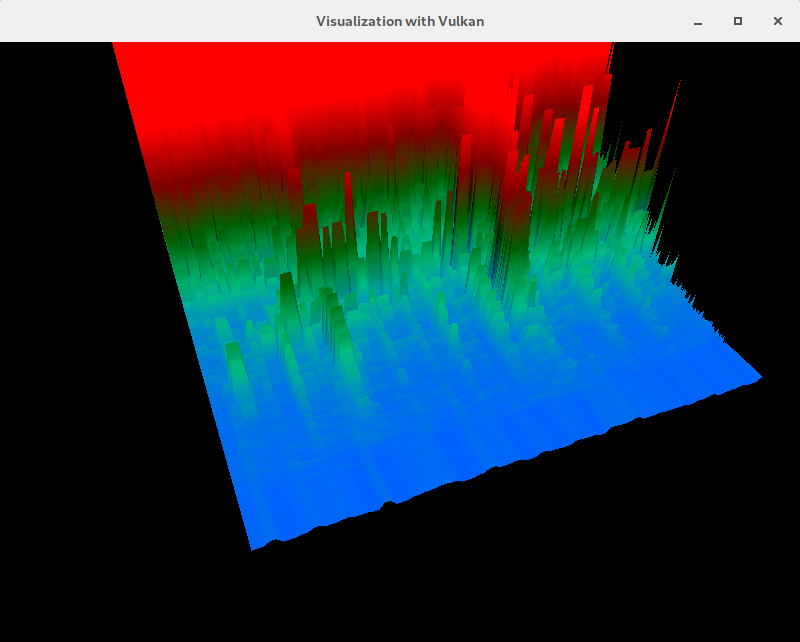
\includegraphics[\width=\textwidth]{img/user/screenshot.png}
	\centering
	\caption{K\'eperny\H ok\'ep a programr\'ol fut\'as k\"ozben.}
\end{figure}
